\documentclass{article}
\usepackage{graphicx}

\begin{document}

\section{Question 1 (10 points)}

\paragraph{1.} Code a function \texttt{Poisson\_Process(lambda,x\_size,y\_size)} that generates a Poisson point process of intensity $\lambda$ in a window of size $x\_size\times y\_size$.

\paragraph{2.} Code a function \texttt{Count\_Pairs(X,R)} that counts the number of pairs of points in a set $X$ located at a distance less than $R$.\\

We want to implement a function that returns a Strauss-like point process. A Strauss process is based on iterations upon a constrained\footnote{A constrained Poisson process has a fixed number of points which doesn't follow on a Poisson law anymore.} Poisson process in a window of size $[0;1]\times[0;1]$, where $X_0$ will denote the initial set of points. At each iteration, one of the points is slightly moved (e.g. according to a normal distribution of low variance). We then consider the quantity $\alpha$ defined as follows.

\begin{enumerate}
\item[•] If the point leaves the observation window, it returns to its initial position, i.e. $\alpha=0$.
\item[•] If \texttt{Count\_Pairs(X$_{n+1}$,R)} is less than \texttt{Count\_Pairs(X$_{n}$,R)}, with $X_n$ the set of points at the iteration $n$ and $R$ a parameter of the process, then $\alpha=1$.
\item[•] Else $\alpha =\gamma^{\left(\texttt{Count\_Pairs}(X_{n+1},R)-\texttt{Count\_Pairs}(X_{n},R)\right)}$, with $\gamma$ a parameter of the process.
\item[•] Finally, a number $\beta$ is drawn randomly between 0 and 1. If $\beta<\alpha$, then the point set is updated with the shifted element. Otherwise, the original set is retained.
\end{enumerate}

\paragraph{3.} Code a function \texttt{Strauss(n,gamma,R,N} that generates a Strauss point process of $n$ points and with parameters $\gamma\in[0;1]$, $R>0$ and $N$ the number of iterations.


\begin{enumerate}
\item[\textbf{a.}] Test your \texttt{Strauss(lambda,gamma,R,N} function with $n=100$, $\gamma = 0.1$, $R=0.2$ and $N\geq 1000$.
\item[\textbf{b.}] Test your \texttt{Strauss(lambda,gamma,R,N} function with $n=100$, $\gamma = 0.1$, $R=0.05$ and $N\geq 1000$.
\item[\textbf{c.}] What happens if $\gamma = 1$?
\end{enumerate}

\paragraph{6.} How could you both  quantitatively and qualitatively characterise the different point process you can generate with this function? (Bonus: do it.)\\




Useful Python function: \texttt{scipy.spatial.distance.pdist}.\\

Useful MATLAB function	: \texttt{pdist}.




















\newpage

\section{Question 2 (10 points)}
Let us consider a set of binary images made of white particles on a black background. The particles are disks or ellipses of random radius.

\begin{center}
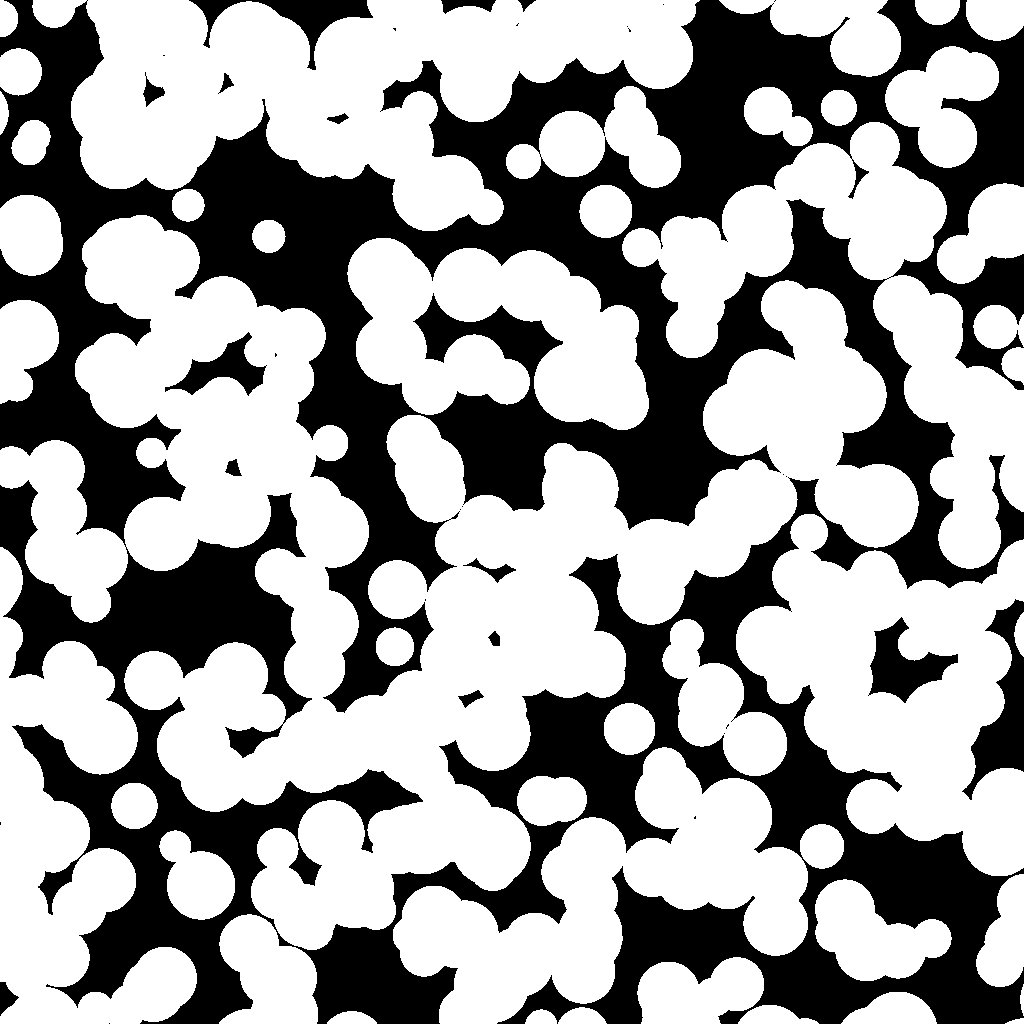
\includegraphics[width=.4\textwidth]{I_400_2.png}
\qquad
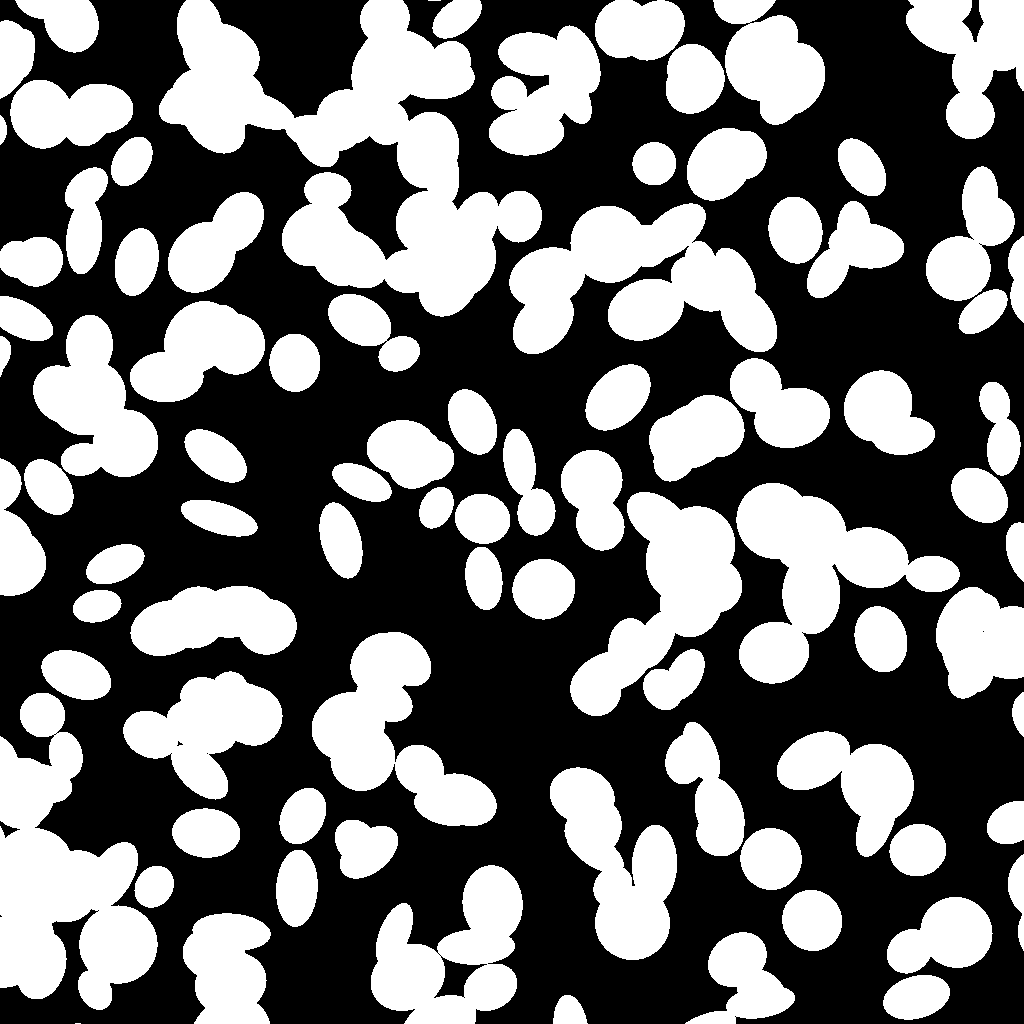
\includegraphics[width=.4\textwidth]{I_250_7.png}
\end{center}

Propose and implement a method to retrieve the characteristics of the mean particle for each set of images at your disposal: area, perimeter and mean radius for disks; mean equivalent radius for ellipses. \\

Explain your methodology and any assumptions you may have to make.\\


Useful Python functions: \texttt{skimage.measure.area}, \texttt{skimage.measure.perimeter}, \texttt{skimage.measure.euler\_number}, \texttt{scipy.optimize.fmin}.\\

Useful MATLAB functions: \texttt{bwarea}, \texttt{bwperim}, \texttt{bweuler}, \texttt{fminsearch}.




\end{document}